In this section, we present our measurement methodology along with the
metrics considered and discuss energy efficiency and power-performance
traces of the model system.

\subsection{Measurement methodology}
\label{subsec:4.1}

We  approach  the  assessment  of  the energy  footprint  and  overall
performance   of   \cosmoart   with  two   important  metrics:
\textit{time-to-solution} (TTS) and \textit{energy-to-solution} (ETS).
TTS refers to  the total wall clock time  of the application execution
time. ETS  is the amount of  energy spent to  achieve results.  Energy
consumption  is  assessed by  sampling  the  instantaneous peak  power
during execution which  is then averaged and multiplied  by the TTS to
determine  ETS.   Whenever  possible,  multiple production  runs  were
performed  to  illustrate the  reproducibility  of  the baseline,  and
quantify the  significant uncertainties  in the power  measurement, as
dictated by the available technology.

\subsection{Time-power-energy analysis of \textsc{Cosmo-art}}
\label{subsec:4.2}

\begin{figure}[htbf]
  \begin{center}
    \includegraphics[width=0.48\textwidth]{Figs/NRJ_benchmark_Monch.eps}
    \caption{\textsc{Monch}: Isola E1 Rack 2 Total Power}
    \label{fig:1}
  \end{center}
\end{figure}

\begin{figure}[htbf]
  \begin{center}
    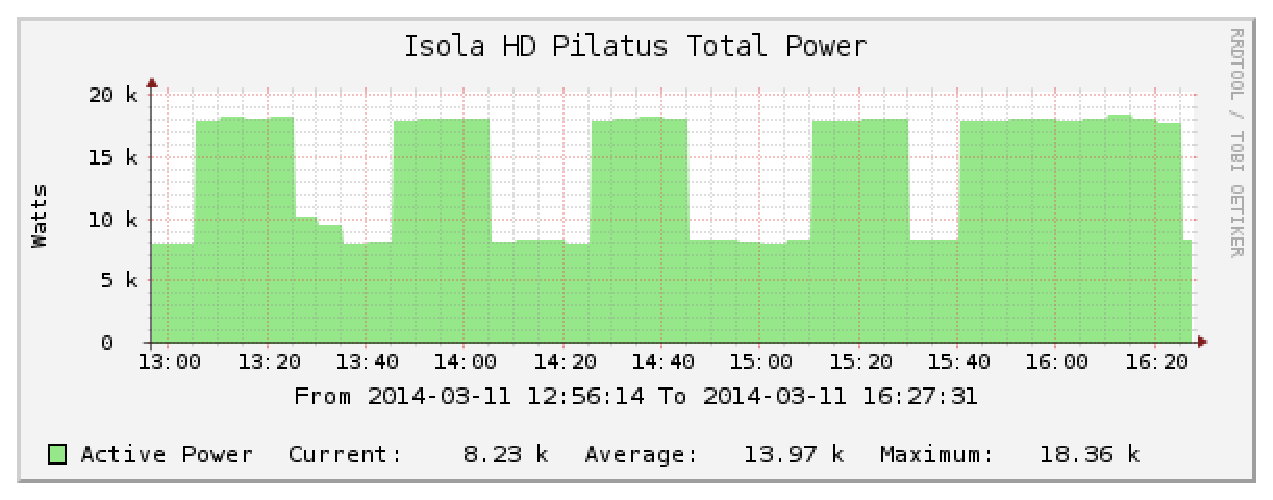
\includegraphics[width=0.48\textwidth]{Figs/NRJ_benchmark_Pilatus.eps}
    \caption{\textsc{Pilatus}: Isola HD Total Power}
    \label{fig:2}
  \end{center}
\end{figure}

Figures~\ref{fig:1}   and   \ref{fig:2}   account   respectively   for
\textsc{Monch}'s Isola E1 Rack  2 and \textsc{Pilatus}' Isola HD total
power measurements for  1-day or 2-days simulations. On  the Intel Ivy
Bridge EP  based cluster (i.e.  \textsc{Monch}),  the 1-day simulation
was issued  only twice due  to usage restrictions. As  time resolution
was set to one update every  5 minutes for power sampling, the average
power consumption was computed by considering 6 values for each single
run.  On the Intel Xeon E5 based cluster (i.e.  \textsc{Pilatus}), the
1-day simulation  was issued  four times and  a 2-days run  only once.
Similarly, the average power consumption was computed by considering 4
values  for  each  single  1-day  run  and 9  values  for  the  2-days
run. Corresponding results are gathered in Table~\ref{tab:3}.

\begin{table}[htbf]
  \begin{center}
    \caption{Average power consumption (W) of the platforms}
    \label{tab:3}
    \begin{tabular}{cccc}
      \hline\noalign{\smallskip}
      \textbf{\scriptsize{Xeon E5}} & \textbf{\scriptsize{Ivy Bridge}} & \textbf{\scriptsize{Xeon  E5645}} & \textbf{\scriptsize{Xeon  E5645}}\\
      & & \textbf{\scriptsize{(Polling)}} & \textbf{\scriptsize{(Blocking)}} \\
      \noalign{\smallskip}\hline\noalign{\smallskip}
      18035.0 & 12622.5 & 3713.6 & 3651.8 \\ 
      \noalign{\smallskip}\hline
    \end{tabular}
  \end{center}
\end{table}

In  Figure~\ref{fig:3}, we  compare both  TTS (right  y-axis)  and ETS
(left  y-axis)  metrics  on  both  platforms.  As  expected,  Xeon  E5
outperforms Ivy Bridge EP, being  roughly 1.3x faster.  The reason for
that is  two-fold: (1) it has  higher clock frequency  than Ivy Bridge
(2.6  GHz  against  2.2 GHz),  and  (2)  it  aims at  computing  speed
regardless to  energy consumption.  In our experiments,  Ivy Bridge EP
showed the best energy-to-solution, reducing the energy consumption of
Xeon E5 by approximately $7\%$.

\begin{figure}[htbf]
  \includegraphics[width=0.5\textwidth]{Figs/Time_E2S_COSMO-ART-0.eps}
  \caption{Time-to-solution and energy-to-solution comparison between
    Xeon E5 and Ivy Bridge-EP architectures for a 24h simulation}
  \label{fig:3}
\end{figure}

\begin{figure}[htbf]
  \includegraphics[width=0.5\textwidth]{Figs/Time_E2S_COSMO-ART-5.eps}
  \caption{Mean time-to-solution and energy-to-solution on
    \textsc{Tintorrum} for a 24h simulation - MPI Polling and Blocking
    modes}
  \label{fig:4}
\end{figure}

\subsection{Power-performance tracing of \textsc{Cosmo-art}}
\label{subsec:4.3}

\begin{figure*}[htbf]
  \centering
  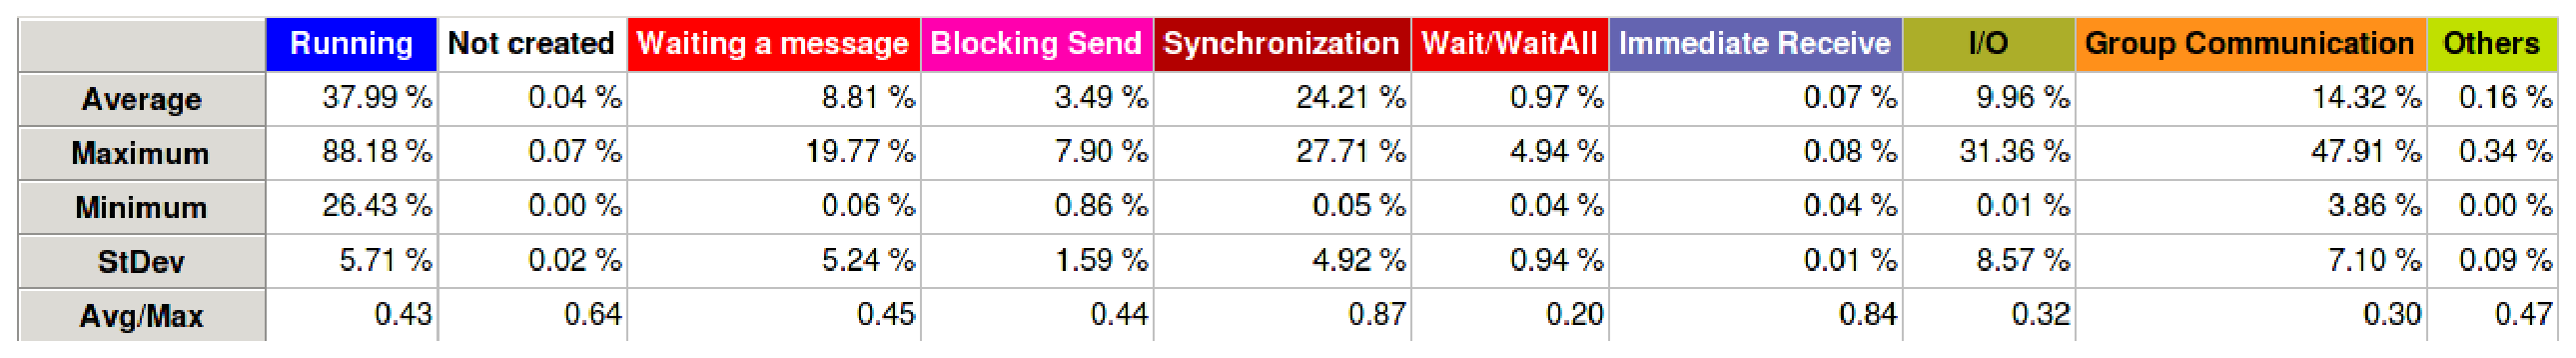
\includegraphics[width=0.78\textwidth]{Figs/23_24_blq1_stat1.eps}
  \caption{blabla}
  \label{fig:8}
\end{figure*}

\begin{figure*}[htbf]
  \centering
  \scalebox{0.5}{\input{Figs/24hour.pstex_t}}
  \caption{24 hours simulation trace using the MPI blocking mode on
    \textsc{Tintorrum}.}
  \label{fig:9}
\end{figure*}

\begin{figure*}[htbf]
  \centering
  \scriptsize
  MPI polling mode\\
  \scalebox{0.5}{\input{Figs/11_12_blq0_figure.pstex_t}}\\
  MPI blocking mode\\
  \scalebox{0.5}{\input{Figs/11_12_blq1_figure.pstex_t}}\\
  MPI polling mode\\
  \scalebox{0.5}{\input{Figs/23_24_blq0_figure.pstex_t}}\\
  MPI blocking mode\\
  \scalebox{0.5}{\input{Figs/23_24_blq1_figure.pstex_t}}\\
  \caption{1 hour simulation (23h-24h) trace using the MPI blocking
    mode on \textsc{Tintorrum}.}
  \label{fig:11}
\end{figure*}
